\documentclass{beamer}
\mode<presentation>
{ \usetheme{boxes} }

\usepackage{times}
\usepackage{graphicx}
\usepackage[backend=bibtex]{biblatex}

\newcommand{\etal}{\textit{et al}. }
\newcommand{\ie}{\textit{i}.\textit{e}., }
\newcommand{\eg}{\textit{e}.\textit{g}. }
\newcommand{\etc}{\textit{etc}. }

\title{An Introduction to Model Driven Engineering}
\author{Marco Craveiro}
\date{\today}

\AtBeginSection[]
{
  \begin{frame}<beamer>
    \frametitle{Outline}
    \tableofcontents[currentsection]
  \end{frame}
}

\bibliography{an_introduction_to_mde}

\begin{document}

\begin{frame}
\titlepage
v${DOGEN_VERSION}
\end{frame}

\section{Historical Context}

\begin{frame}
\frametitle{Historical Context}

The software industry has had to deal with two big problems, both
related to reducing the role of humans in the software development
process:
\pause

\begin{itemize}
\item How to lower the cost of development and maintenance of systems
  via automation:
  \pause

  \begin{itemize}
  \item All of the software engineering that can be reduced to a
    machine understandable representation should be automated.
    \pause
  \item Humans should be used only where they add value.
    \pause
  \end{itemize}

\item How to extract the domain essence of legacy systems such that
  they can be moved across from legacy platforms into newer platforms.
\end{itemize}

\end{frame}

\begin{frame}
\frametitle{Historical Context}

Whilst pursuing these, the industry bumped into two core concepts:
\pause

\begin{itemize}
\item \emph{Platform Independent Models}: (PIMs) The portion of the
  domain knowledge in a system which is not directly related to a
  specific implementation.
  \pause

\item \emph{Platform Specific Models}: (PSMs) The portion of the
  system which is specific to a platform.
\end{itemize}

\pause

The holy grail was then to extract a PSM from an existing system, and
then use it to generate PSMs. This required a theoretical foundation
on which to build this work.

\end{frame}

\section{Models and Modeling}

\begin{frame}
\frametitle{Models and Modeling}

One of the first stumbling blocks is a suitable definition of a
Model:
\pause

\begin{itemize}
\item It is a very general term which raises deep philosophical
  questions.
  \pause
\item We need to set some boundaries in terms of what we are trying to
  achieve.
  \pause
\end{itemize}

Brambilla \cite{brambilla2012model}:

\begin{quote}
We are not interested here by a theoretical definition of a model, but
by an engineering one, \ie a definition that will help users to
implement and maintain systems.
\end{quote}

\end{frame}

\begin{frame}
\frametitle{Models and Modeling}

Brambilla\cite{brambilla2012model} states:

\begin{quote}
We can informally define a model as a simplified or partial
representation of reality, defined in order to accomplish a task or to
reach an agreement on a topic. Therefore, by definition, a model will
never describe reality on its entirety.
\end{quote}

\pause

On the paper, Beziven states:

\begin{quote}
[\ldots] [A] graph-based structure representing some aspects of a
given system and conforming to the definition of another graph called
the meta-model. [\ldots] A model is said to \textbf{represent} a
system.
\end{quote}

\pause

V{\"o}elter \etal~\cite{volter2013model} state:

\begin{quote}
A model is an abstract representation of a system’s structure,
function or behavior.
\end{quote}

\end{frame}

\begin{frame}
\frametitle{Models and Modeling}

\begin{itemize}
\item ``The model always exists, the only option designers have is
  about its form: it may be mental (existing only in the designers
  head) or explicit.\cite{brambilla2012model}
  \pause
\item There are many kinds of models: sketches, blueprints, diagrams,
  the programs themselves (modeling the world).
  \pause
\item We are interested in a special class of models: those which are
  described according to a formal language and thus have precise
  semantics.
\end{itemize}

\end{frame}

\begin{frame}
\frametitle{Models and Modeling}

Formal models are written using a DSL (Domain Specific Language). The
DSL is designed specifically for modeling. UML is an example of such a
DSL. UML has a graphical representation, but also an \emph{abstract
  syntax}.

\begin{center}
  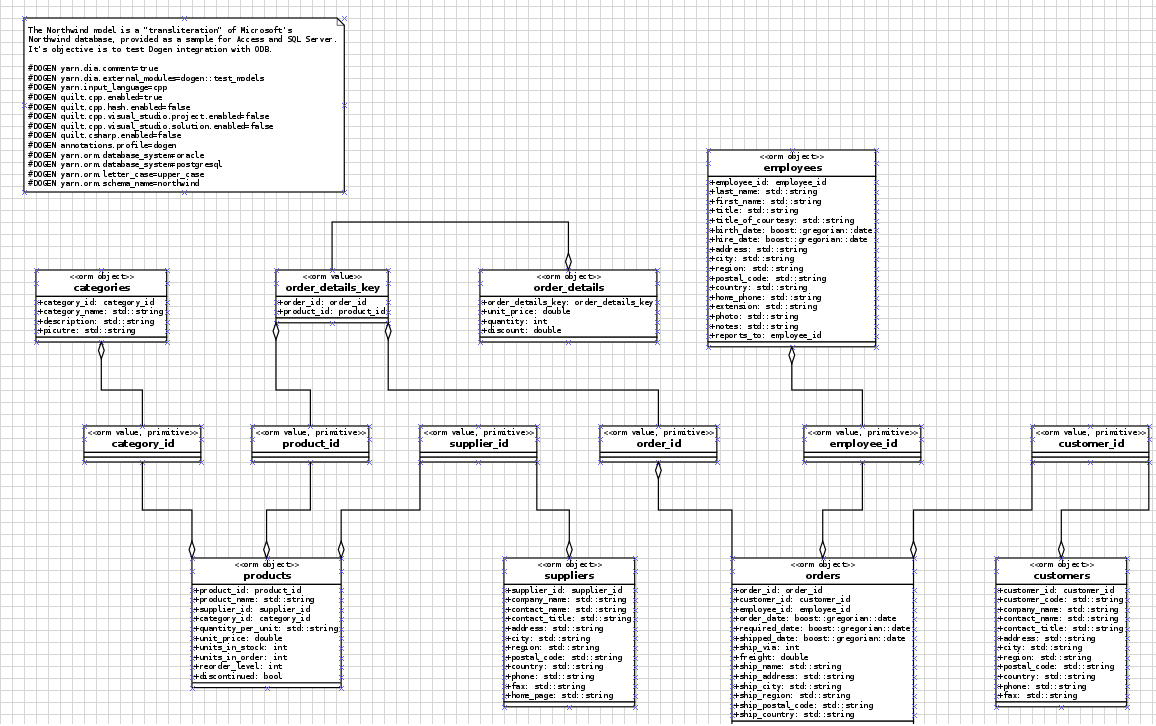
\includegraphics[scale=0.2]{images/northwind_diagram.png}
\end{center}

\end{frame}

\begin{frame}
\frametitle{Models and Modeling}

\begin{itemize}
\item Modeling is thus the process of creating models for a system.
  \pause
\item These are not just \emph{pretty pictures} but formal,
  fundamental knowledge about the system, just like code, but at a
  higher level of abstraction.
  \pause
\item These models contain enough knowledge to create some aspects of
  the system~--- \ie using code generation, we can transform a formal
  model into code.
\end{itemize}

\end{frame}

\section{Model Driven Engineering}

\begin{frame}
\frametitle{Model Driven Engineering}

We can now start to sketch a broad definition of Model Driven
Engineering:
\pause

\begin{itemize}
\item ``Development paradigm that uses models as the primary artifact
  of the development process. Usually [\ldots] the implementation is
  (semi-)automatically generated from the
  models.''\cite{brambilla2012model}
  \pause
\item ``Goes beyond the pure development activities and encompasses
  other model-based tasks of a complete software engineering process
  (\eg the model-based evolution of the system or the model-driven
  reverse engineering of a legacy system.''\cite{brambilla2012model}
\end{itemize}

\end{frame}

\begin{frame}
\frametitle{Model Driven Engineering}

Wirth stated\cite{Wirth:1978:ADS:540029}:

\begin{quote}
  Algorithms + Data Structures = Programs
\end{quote}

\pause

MDE states\cite{brambilla2012model}:

\begin{quote}
  Models + Transformations = Software
\end{quote}

\pause

And then MDE goes even further:

\begin{quote}
  \textbf{Everything} is a model.
\end{quote}

\pause

\begin{itemize}
\item Thus transformations themselves are models;
  \pause
\item The formal language we use to describe models themselves is a
  model.
\end{itemize}

\end{frame}

\section{Meta-Models}

\begin{frame}
\frametitle{Meta-Models}

\begin{itemize}
\item A meta-model is simply a kind of model used to define a
  language to define other models.
  \pause
\item Meta-models are very common in programming; we are just not used
  to thinking about them explicitly.
  \pause
\item All programming languages define meta-models: constructs such
  class, function and so forth are meta-constructs. Users then define
  their own classes, which are instances of this meta-class. Those
  classes are in turn instantiated into objects.
\end{itemize}

\end{frame}

\begin{frame}
\frametitle{Meta-Models}

Other examples of meta-models:

\begin{itemize}
  \item UML is a meta-model with constructs such as class,
    association, attributes and so forth. User models are instances of
    the UML meta-model.
    \pause
  \item XML documents can have an associated XML schema.
    \pause
  \item The RDBMS model has a meta-model composed of tables, columns
    and so forth.
    \pause
  \item NeuroML defines a meta-model to which all instance models
      must conform to in order to be valid NeuroML documents.
\end{itemize}

\end{frame}

\begin{frame}
\frametitle{Meta-Models}

But why bother defining a meta-model explicitly?
\pause

\begin{itemize}
  \item The key point is the second term on our equation:
    transformations.
    \pause
  \item Once we have two explicit meta-models we can create a language
    that describes transformations between those two and automate the
    process.
    \pause
  \item For example, we could create a transformation between an XML
    document and a database schema, generating the tables
    automatically.
\end{itemize}

\end{frame}

\begin{frame}
\frametitle{Meta-Meta-Models}

But is it turtles all the way up?
\pause

\begin{itemize}
  \item If meta-models are formal models, they must also conform to a
    DSL of some kind.
    \pause
  \item Models that are used to define meta-models are called
    meta-meta-models. An example is MOF, the meta-meta-model used to
    define UML.
    \pause
  \item Meta-meta-models are useful in practice because we can use
    them to help define transformations.
    \pause
  \item However, there is no point in going up the abstraction ladder:
    meta-meta-models can be used to define themselves, thus closing
    the process.
\end{itemize}

\end{frame}

\begin{frame}
\frametitle{Meta-Meta-Models}

\begin{center}
  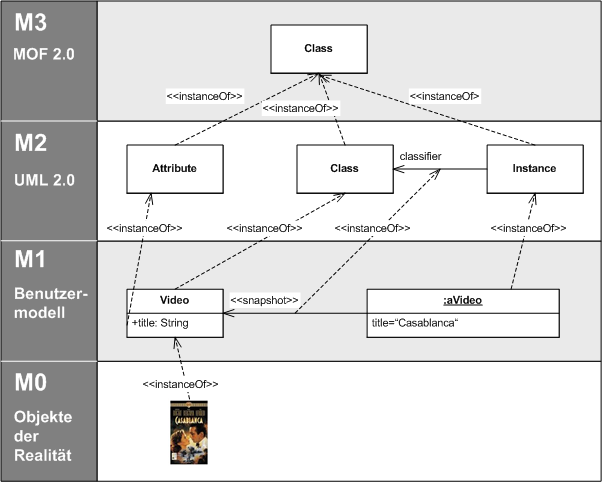
\includegraphics[scale=0.4]{images/uml-m0-m3-wikipedia.png}
\end{center}

\end{frame}

\begin{frame}
\frametitle{Technical Spaces}

To create a bridge between different technologies, the notion of a
Technical Space was introduced\cite{kurtev2002technological}.

\begin{quote}
A technical space is a working context with a set of associated
concepts, body of knowledge, tools, required skills, and
possibilities. It is also a model management framework usually based
on some algebraic structures like trees, graphs, hypergraphs,
categories, \etc Although technical spaces may be difficult to define
formally, they can be easily recognized (e.g. XML, MDA). In the
three-level conjecture, each technical space can be seen as based on a
metametamodel (explicit or implicit) and a collection of metamodels.
\end{quote}

\end{frame}

\begin{frame}
\frametitle{Technical Spaces}

\begin{itemize}
\item Technical Spaces are effectively a package of meta-meta-model, a
  set of meta-models and the associated models one can create from
  them.
  \pause
\item For example, Java and other languages are Technical Spaces,
  and so is XML.
  \pause
\item Technical Spaces provide context to terminology: when you say
  ``model'', it only has meaning in the context of a precise
  Technical Space such as UML or NeuroML \etc.
\end{itemize}

\end{frame}

\begin{frame}
\frametitle{Technical Spaces}

\begin{itemize}
\item Technical Spaces are also a way to structure the Solution
  Space. Different Technical Spaces have different ``abilities'', so
  it is very useful to convert models from one Technical Space to
  another.
  \pause
\item MDE tools such as Eclipse's EMF provide a Technical Space with
  a complete stack of solutions for MDE, including the definition of
  DSLs, modeling, run-time reflection and so forth.
\end{itemize}

\end{frame}

\section{MDE in practice}
\begin{frame}
\frametitle{MDE in practice}

But these books and papers are from the 1990s and 2000s! Where is MDE
now?
\pause

\begin{itemize}
\item Whilst the theory and tooling of MDE is becoming clearer in academic
  terms, its still not widely adopted in practice.
  \pause
\item As Steven Mellor has been saying since 1985: ``Modeling and
  model-driven engineering will be common place in three years time.''
  \pause
\item MDE is becoming yet another Computer Science elusive holy grail
  like AI.
\end{itemize}

\end{frame}

\begin{frame}
  \frametitle{MDE in practice}

Why is it so elusive?
\pause

\begin{itemize}
\item The theoretical models are not complete; there is still no
  proper mathematical theory behind it.
  \pause
\item Institutions and companies such as OMG, Rational, \etc oversold
  the technology to the point of hype and now it has been somewhat
  discredited, as with AI.
\end{itemize}

\end{frame}

\begin{frame}
  \frametitle{MDE in practice}

Why is it so elusive?

\begin{itemize}
\item The theory is very complex and hard to see how it is applied
  until one starts using it. Many people view it as a ``purist
  approach'' that works in theory but is not feasible in practice.
  \pause
\item There is pressure to lower development costs by requiring less
  specialised knowledge so that Software Engineering work can be
  outsourced and off-shored; MDE requires very specialised knowledge
  to get up and running.
  \pause
\item The tooling is not yet mature; it is complex and does not work
  for all use cases; it is common for one to start adopting a
  technology only to find it deficient half-way through adoption.
\end{itemize}

\end{frame}

\begin{frame}
\frametitle{MDE in practice}

My objective is to apply the MDE approach to the Computational
Neuroscience software. This entails:

\begin{itemize}
\item Creating an inventory of systems, simulators, DSLs and
  approaches and a taxonomic classification for them.
  \pause
\item Use MDE techniques to define Technical Space in which different
  Computational Neuroscience tools can be made to interoperate.
  \pause
\item Study the advantages and disadvantages of a structured approach
  to the problem of transformation applied to a real-world field
  rather than the simplified experiments found in some MDE
  literature.
\end{itemize}

\end{frame}

\begin{frame}
  \printbibliography
\end{frame}

\end{document}
